\documentclass{article}

\title{Interpolacja}
\author{Dominik Lau}

\usepackage{blindtext}
\usepackage{amsmath}
\usepackage[utf8]{inputenc}
\usepackage[polish]{babel}
\usepackage[T1]{fontenc}
\usepackage{listings}
\usepackage{color}
\usepackage{amssymb}
\usepackage{esvect}
\usepackage{graphicx}
\usepackage{hyperref}



\definecolor{dkgreen}{rgb}{0,0.6,0}
\definecolor{gray}{rgb}{0.5,0.5,0.5}
\definecolor{mauve}{rgb}{0.58,0,0.82}

\lstset{frame=tb,
  language=Python,
  aboveskip=3mm,
  belowskip=3mm,
  showstringspaces=false,
  columns=flexible,
  basicstyle={\small\ttfamily},
  numbers=none,
  numberstyle=\tiny\color{gray},
  keywordstyle=\color{blue},
  commentstyle=\color{dkgreen},
  stringstyle=\color{mauve},
  breaklines=true,
  breakatwhitespace=true,
  tabsize=3
}

\graphicspath{ {./media/} }
\begin{document}
\maketitle
\section{Wstęp}
Celem projektu było zaimplementowanie i przeanalizowanie dwóch
algorytmów interpolacji na wybranych profilach wysokościowych - metody wykorzystującej wielomian Lagrange oraz metody z funkcjami sklejanymi trzeciego stopnia.
Do implementacji wykorzystano język $Python$ oraz biblioteki
$matplotib$, $pandas$.
\section{Teoria}
W obu przypadkach zakładamy, że mamy pewien zestaw $n+1$ punktów
\begin{gather*}
	(x_0, y_0) \\
	(x_1, y_1) \\
	...\\
	(x_n, y_n)
\end{gather*}
Chcemy znaleźć taką funkcję $F(x)$, że
\begin{gather*}
	\forall_{i= 0..n}  F(x_i) = y_i
\end{gather*}
dobrze określającą, jakie wartości przyjmują $y$ w punktach $x \notin \{x_0, ..., x_n\}$
\subsection{Metoda Lagrange}
W metodzie tej funkcja $F$ ma postać
\begin{gather*}
	F(x) = \Sigma_{i=0}^{n} y_i \phi_i(x)
\end{gather*}
gdzie 
\begin{gather*}
	\phi_i(x) = \Pi_{j=0,  j \ne i}^{n+1} \frac{x-x_j}{x_i - x_j}
\end{gather*}
jest \textbf{bazą Lagrange'a}. Metoda ta zwraca takie same wyniki
jak metoda Vandermonde, jednak nie musimy rozwiązywać układu równań liniowych
\subsection{Metoda krzywych sklejanych 3. stopnia}
w tej metodzie funkcja $F$ ma postać
\begin{gather*}
	F(x) = S_i(x); x\in [x_i, x_{i+1}]
\end{gather*}
czyli przedstawiamy ją jako szereg połączonych wielomianów $S_i(x)$ takich, że
\begin{gather*}
	deg (S_i) = 3
\end{gather*}
w celu uzyskania układów równań, z których pozyskamy współczynniki $S_i(x)$ przyjmujemy założenia
\begin{gather*}
	S_i(x_i) = y_i \\
	S_i(x_{i+1}) = y_{i+1} \\
	S_{j-1}'(x_i) = S_{j}'(x_i); x = 1..n-1 \\
	S_{j-1}''(x_i) = S_{j}''(x_i); x = 1..n-1 \\
	S_0''(x_0) = 0 \\
	S_{n-1}'' (x_n) = 0 \\
\end{gather*}
znalezienie wielomianów $S$ sprowadza się do rozwiązania powyższego układu równań, w praktyce można wyprowadzić z powyższych układów
wzory na $b,d$ w zależności od $c$ a następnie rozwiązać cały układ równań dla wektora $\textbf{c} = [c_0, ..., c_{n-1}]$:
\begin{gather*}
	\begin{pmatrix}
	1 & 0  & ...  & 0 & 0 \\
	h_1 & 2(h_1 + h_2) & h_2 & 0  & 0 & ... \\
	0 & h_2 & 2(h_2 + h_3) & h_3 & 0 & ... \\
	... \\
	0  & 0 & 0 & ... & 0 & 1
	\end{pmatrix} 
	\begin{pmatrix}
	c_0 \\me
	... \\
	c_{n-1}
	\end{pmatrix}
	= \begin{pmatrix}
		0 \\ 3(\frac{a_2 - a_1}{h_2} - \frac{a_1 - a_0}{h_0}) \\ ... \\ 0
	\end{pmatrix}\\
	d_i = \frac{c_{i+1} - c_i}{3h_i} \\
	b_i = \frac{a_i - a_{i-1}}{h_i} - \frac{h_i}{3}(2c_i + c_{i+1}) \\
\end{gather*}
i właśnie z tak uproszczonego układu skorzystano w implementacji (rozwiązany metodą Jacobiego)
\section{Wybrane profile wysokościowe}
Do analizy wybrano następujące profile wysokościowe
\begin{itemize}
	\item ścieżkę Yoshidy na górę Fuji - jedno duże wzniesienie
	\item Al.  Ujazdowskie-Łazienki-Solec - trasa głównie płaska
	\item wokół centrum Słupska - wiele nagłych (ale niedużych) wzniesień
\end{itemize}
\section{Trasa na górę Fuji}
\begin{center}
	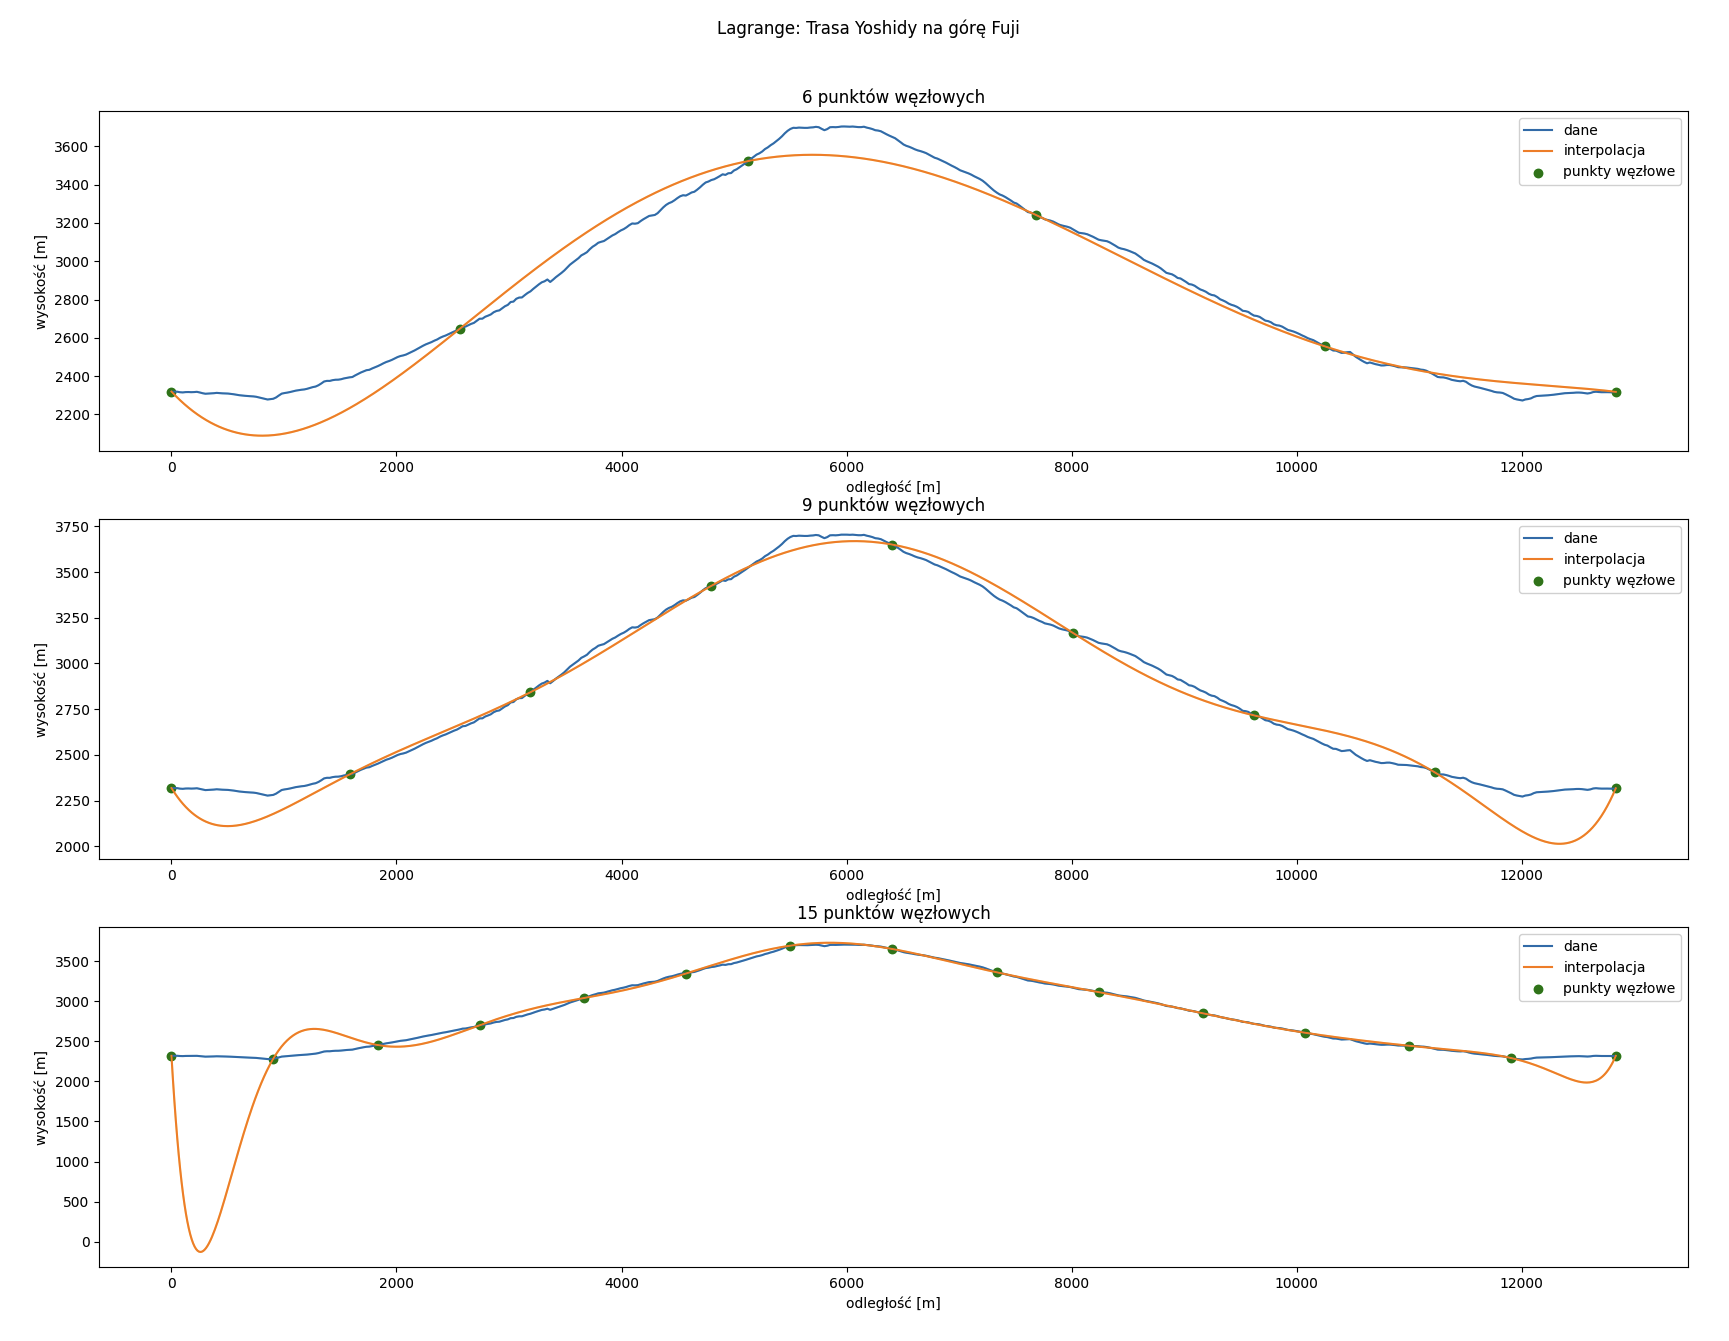
\includegraphics[width=12cm]{lagrange_fuji_uniform}
\end{center}
Na powyższych wykresach widzimy wpływ zwiększania ilości punktów węzłowych rozłożonych równomiernie na jakość wyznaczanych wartości interpolacji. 
Przede wszystkim należy zwrócić uwagę, że dla tej trasy otrzymujemy szybko \textbf{dobre odzwierciedlenie odcinków o stałym nachyleniu}, czyli np.  od 2 do 4 km 
trasy. Problemem jest z nagłym spadkiem lub wzrostem nachylenia, jak w przypadku środka przedziału - dla mniejszej ilości punktów węzłowych \textbf{możemy nie trafić w charakterystyczny punkt zmiany nachylenia} przez co wyznaczone wartości niewiernie będą odzwierciedlały prawdziwą funkcję. Z tym problemem mamy do czynienia
w przypadku 6 i 9 punktów węzłowych. Ponadto w przypadku 15 punktów węzłowych mamy do czynienia z nasileniem innego nieprzychylnego zjawiska, czyli z 
\textbf{efektem Rungego}. Wraz ze wzrostem ilości punktów węzłowych jakość interpolacji na krańcach przedziału pogarsza się (chociaż w środku przedziału obserwujemy 
poprawę). Na redukcję efektu Rungego wpłyniemy poprzez zmianę rozmieszczenia punktów, co zilustrowano poniżej.
 \begin{center}
	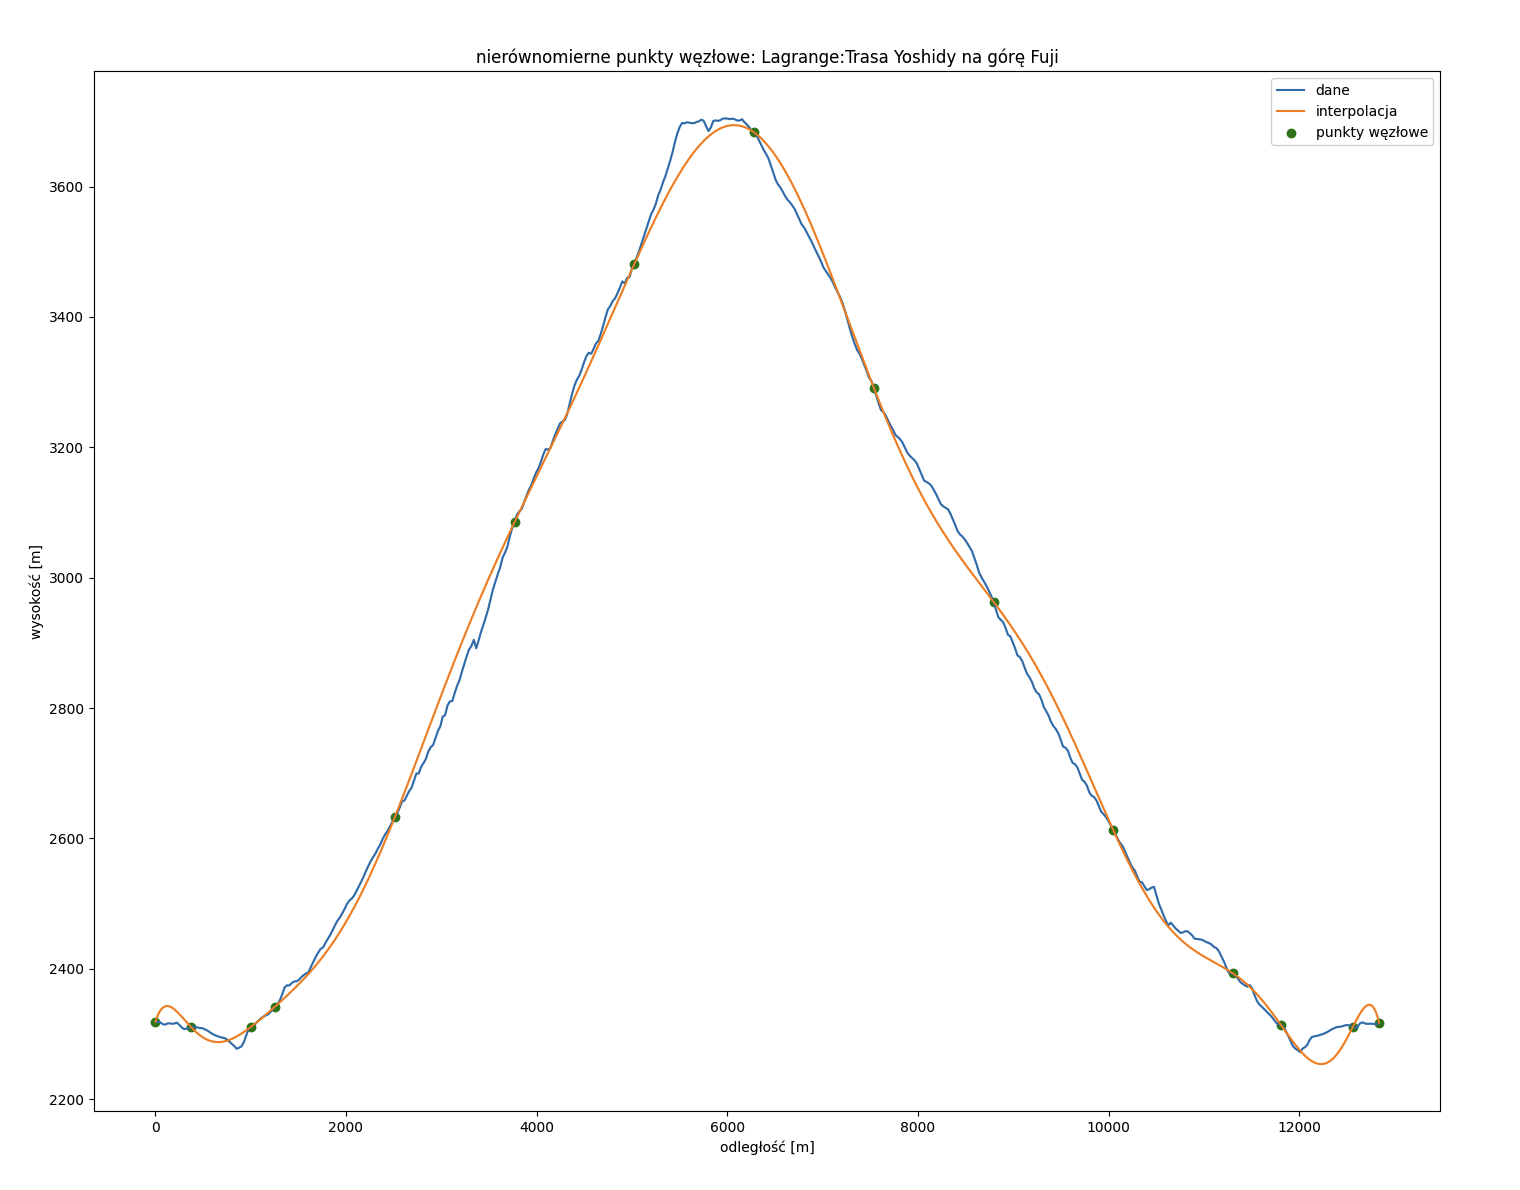
\includegraphics[width=8cm]{lagrange_fuji_runge}
\end{center}
Jak widać rozmieszczając 15 punktów nierównomiernie - \textbf{zwiększamy gęstość na krańcach przedziału} - otrzymujemy znaczne zmniejszenie (chociaż
nie pozbycie się) oscylacji.  Czynimy to kosztem gorszej jakości interpolacji w środku przedziału przy takiej samej złożoności obliczeniowej. Możemy zauważyć
również porównując interpolację z 9 równomiernie rozmieszczonymi punktami do powyższej, że w przypadku nierównomiernego rozmieszczenia w środku przedziału
pojawiają się wahania nawet dla odcinków o stałym nachyleniu. A oto jak z trasą na górę Fuji radzi sobie druga badana metoda
 \begin{center}
	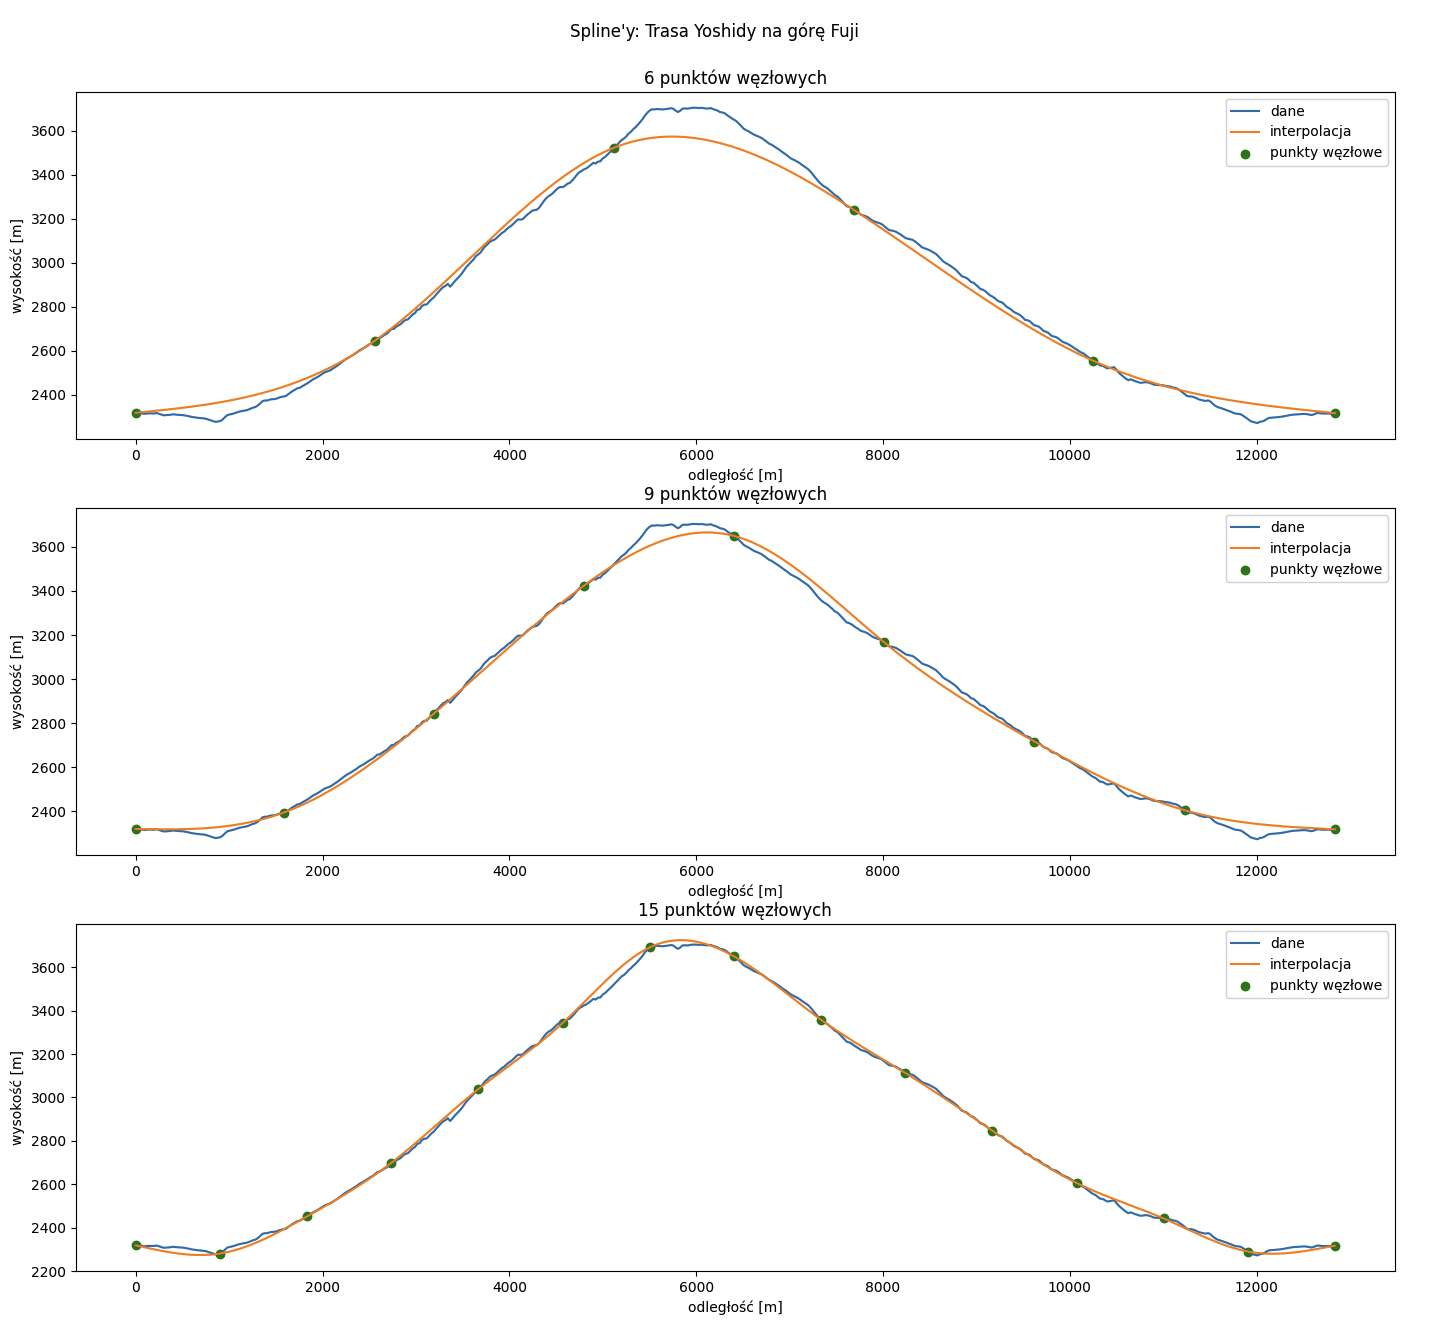
\includegraphics[width=12cm]{spline_fuji_uniform}
\end{center}
Chociaż w tym wypadku dla środka przedziału brak jest dużych różnic w stosunku do metody Lagrange'a, to \textbf{pozbywamy się efektu Rungego}. Tym samym 
dla metody krzywych sklejanych możemy poprawiać jakość interpolacji poprzez zwyczajne zwiększanie punktów węzłowych rozłożonych równomiernie
bez ryzyka pogorszenia aproksymacji na brzegach przedziału.
 \begin{center}
	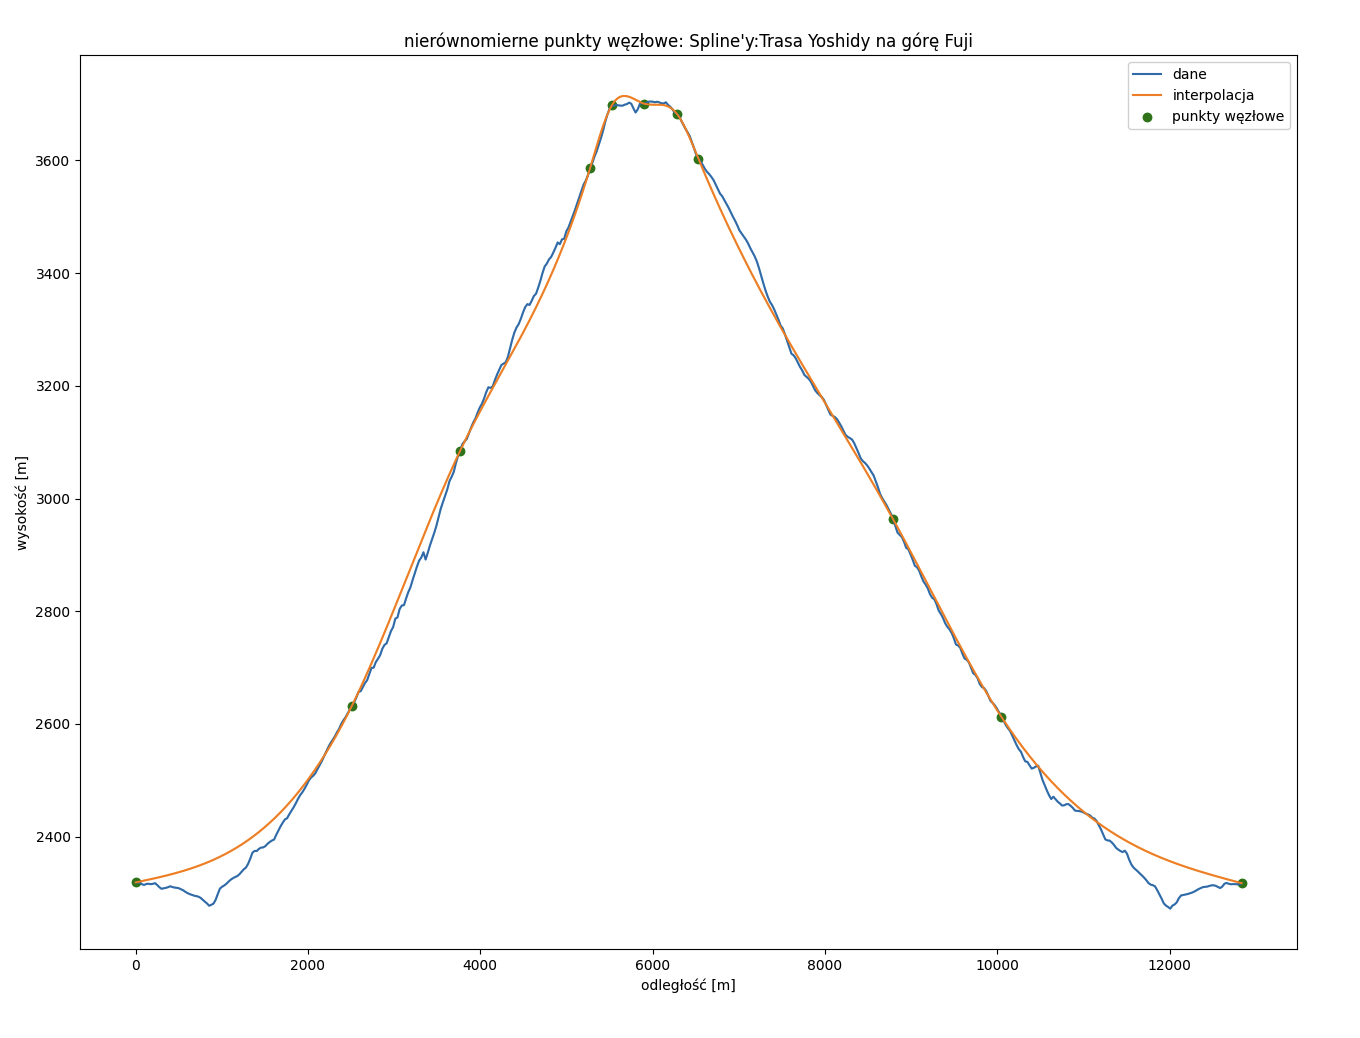
\includegraphics[width=8cm]{spline_fuji_non}
\end{center}
Możemy również próbować w przypadku funkcji sklejanych umieszczać węzły w punktach charakterystycznych, jednak efekt jest podobny jak w przypadku
rozmieszczenia równomiernego, a może nawet prowadzić do gorszej interpolacji w pewnych odcinkach.
\section{Trasa w Warszawie}
 \begin{center}
	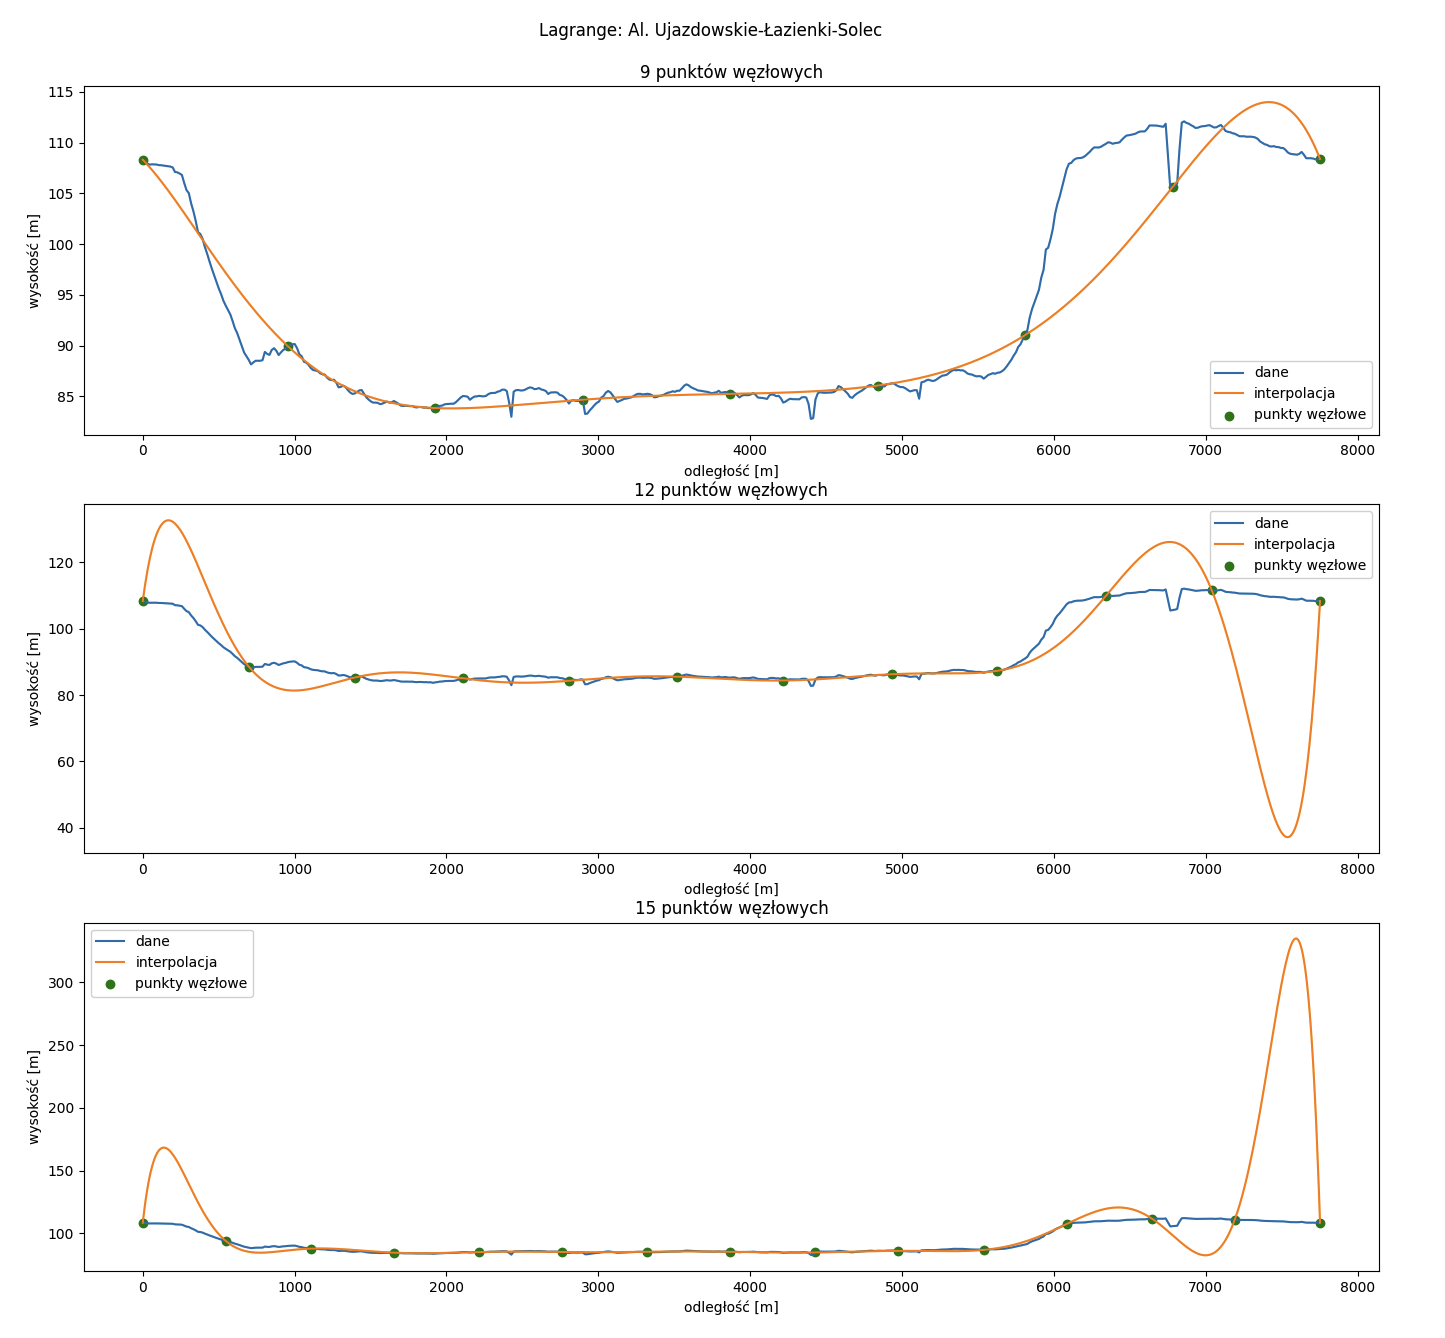
\includegraphics[width=12cm]{lagrange_wwa_uniform}
\end{center}
Przedstawiona trasa jest płaska (drobne spadki i wzniesienia $\sim$ 2m) z dwoma znacznymi wzniesieniami. Dla interpolacji wielomianowej w przypadku 
9 punktów mamy dobre odwzorowanie przebiegu funkcji dla terenu płaskiego (pomijając wspomniane wcześniej drobne spadki), natomiast ze względu na
kłopotliwe umiejscowienie węzłów w okolicach wzniesień krzywa mniej wiernie odwzorowuje profil terenu.  Występuje przypadek analogiczny do widzianego
w przypadku góry Fuji - \textbf{jakość interpolacji dla nagłych wzniesień mocno zależy od rozmieszczenia punktów}, natomiast tereny płaskie są ogółem dobrze odzwierciedlane i rozmieszczenie punktów nie gra tak istotnej roli.  Jeżeli chcemy otrzymać lepszą interpolację to w tym wypadku efekt Rungego pojawia się
bardzo szybko, ponieważ już dla 12 punktów węzłowych mamy znaczne odchylenia od oczekiwanej wartości funkcji (w pewnych miejscach wynik nawet dwukrotnie większy).
Efekt podobnie jak w przypadku profilu góry Fuji nasila się wraz ze wzrostem ilości punktów węzłowych. Ostatecznie \textbf{dla równomiernie rozmieszczonych węzłów
metodą Lagrange'a nie jesteśmy w stanie uzyskać dobrej interpolacji dla tego terenu}.  Wcześniej zwiększaliśmy gęstość węzłów na brzegach przedziału. Co jeśli 
większość punktów skumulujemy w jego środku?
 \begin{center}
	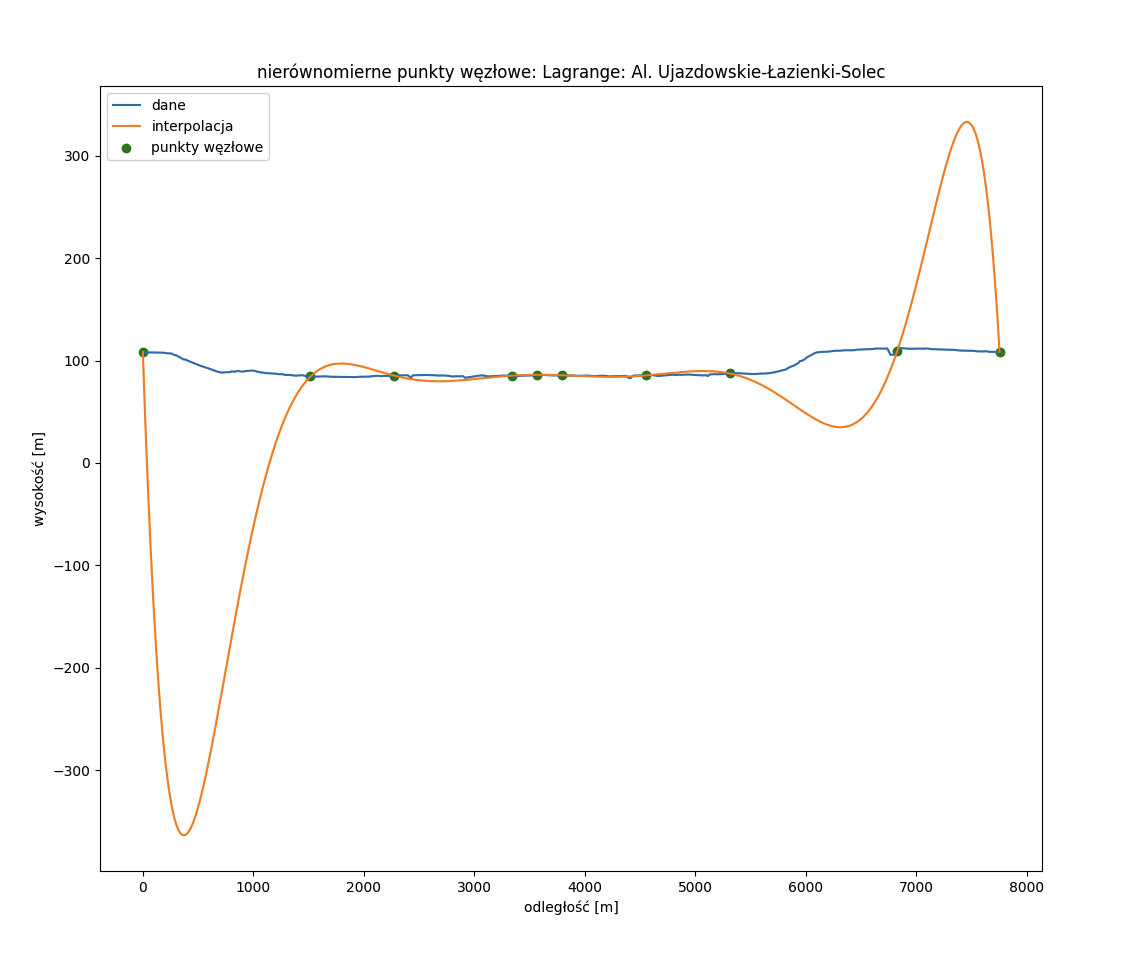
\includegraphics[width=8cm]{lagrange_wwa_runge_magnified}
\end{center}
\textbf{Dla mniejszej ilości punktów węzłowych efekt Rungego został spotęgowany}. Możemy zatem wnioskować, że jego skala jest związana z względną gęstością punktów
w środku i na obrzeżu przedziału. Dla porównania próba redukcji efektu:
 \begin{center}
	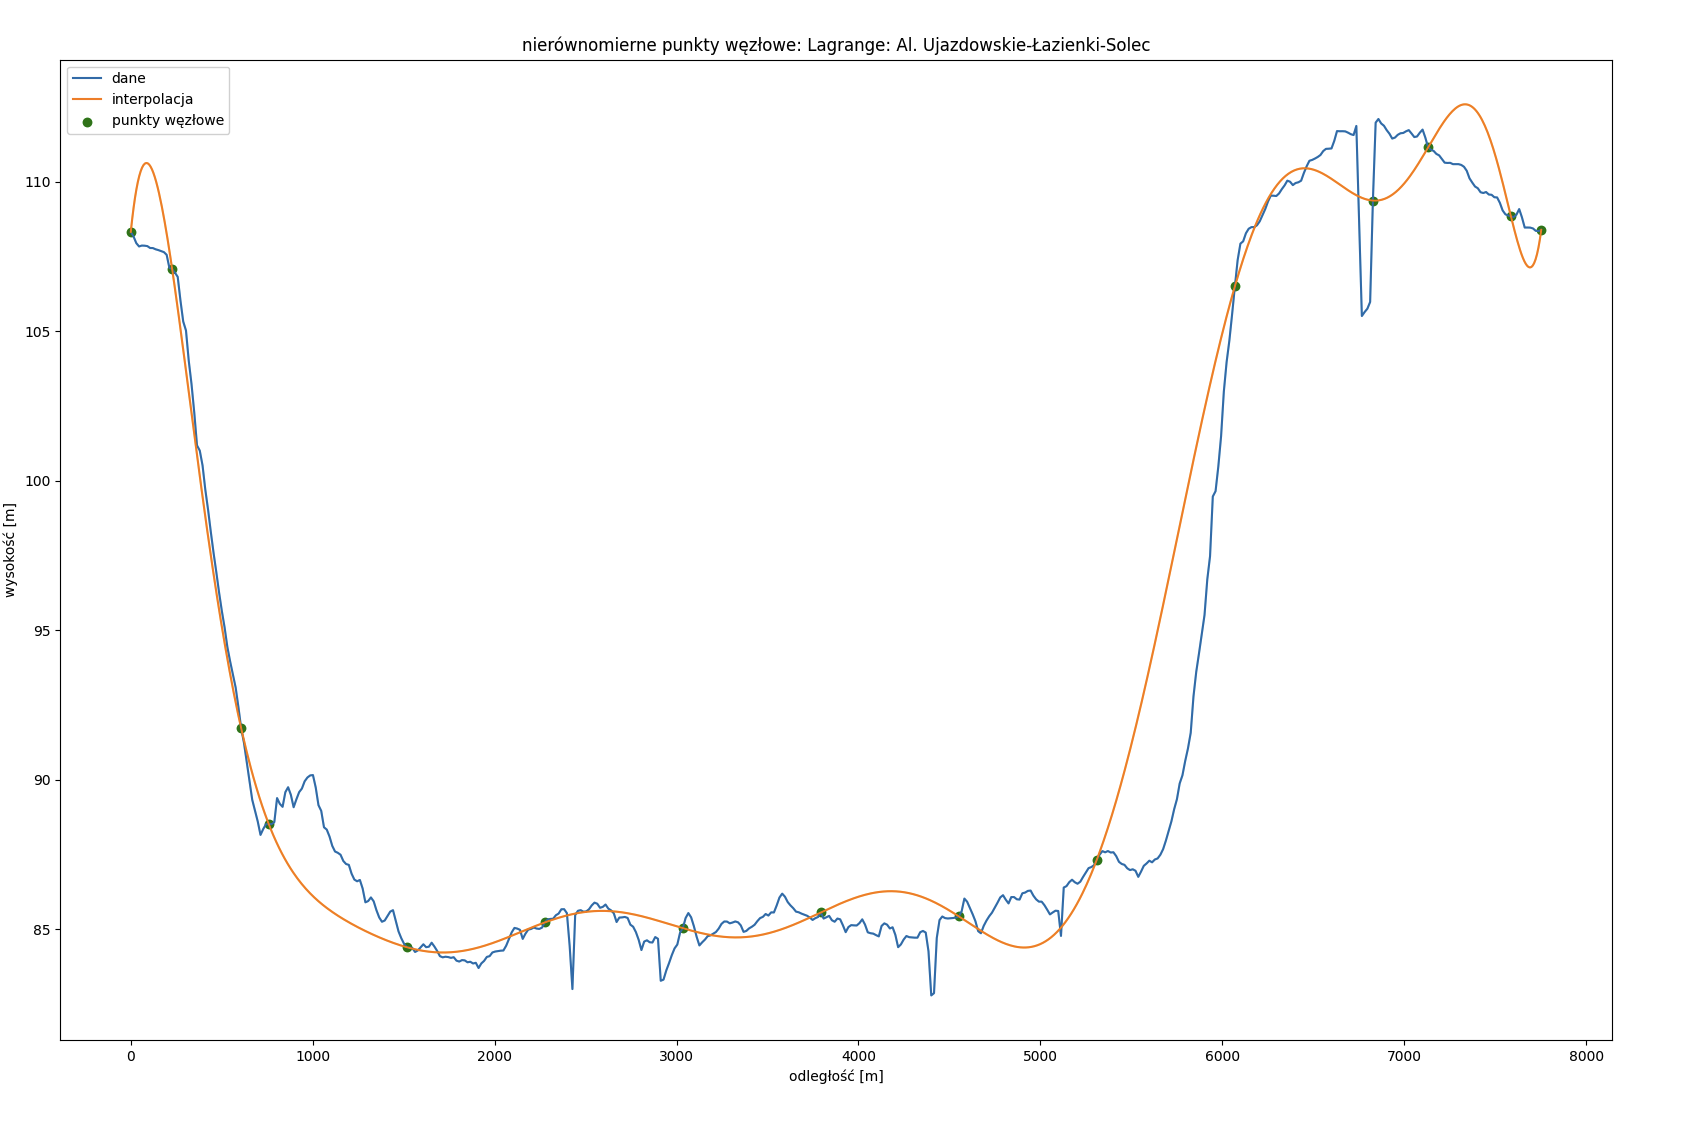
\includegraphics[width=8cm]{lagrange_wwa_runge}
\end{center}
Dla tak rozmieszczonych 15 punktów węzłowych \textbf{efekt jest lepszy niż gdy rozmieściliśmy je równomiernie}. 
Niemniej jednak środek przedziału nie jest wiernie odwzorowany, zupełnie tak jak w przypadku góry Fuji, teraz jednak te odstępstwa są bardziej widoczne.
 \begin{center}
	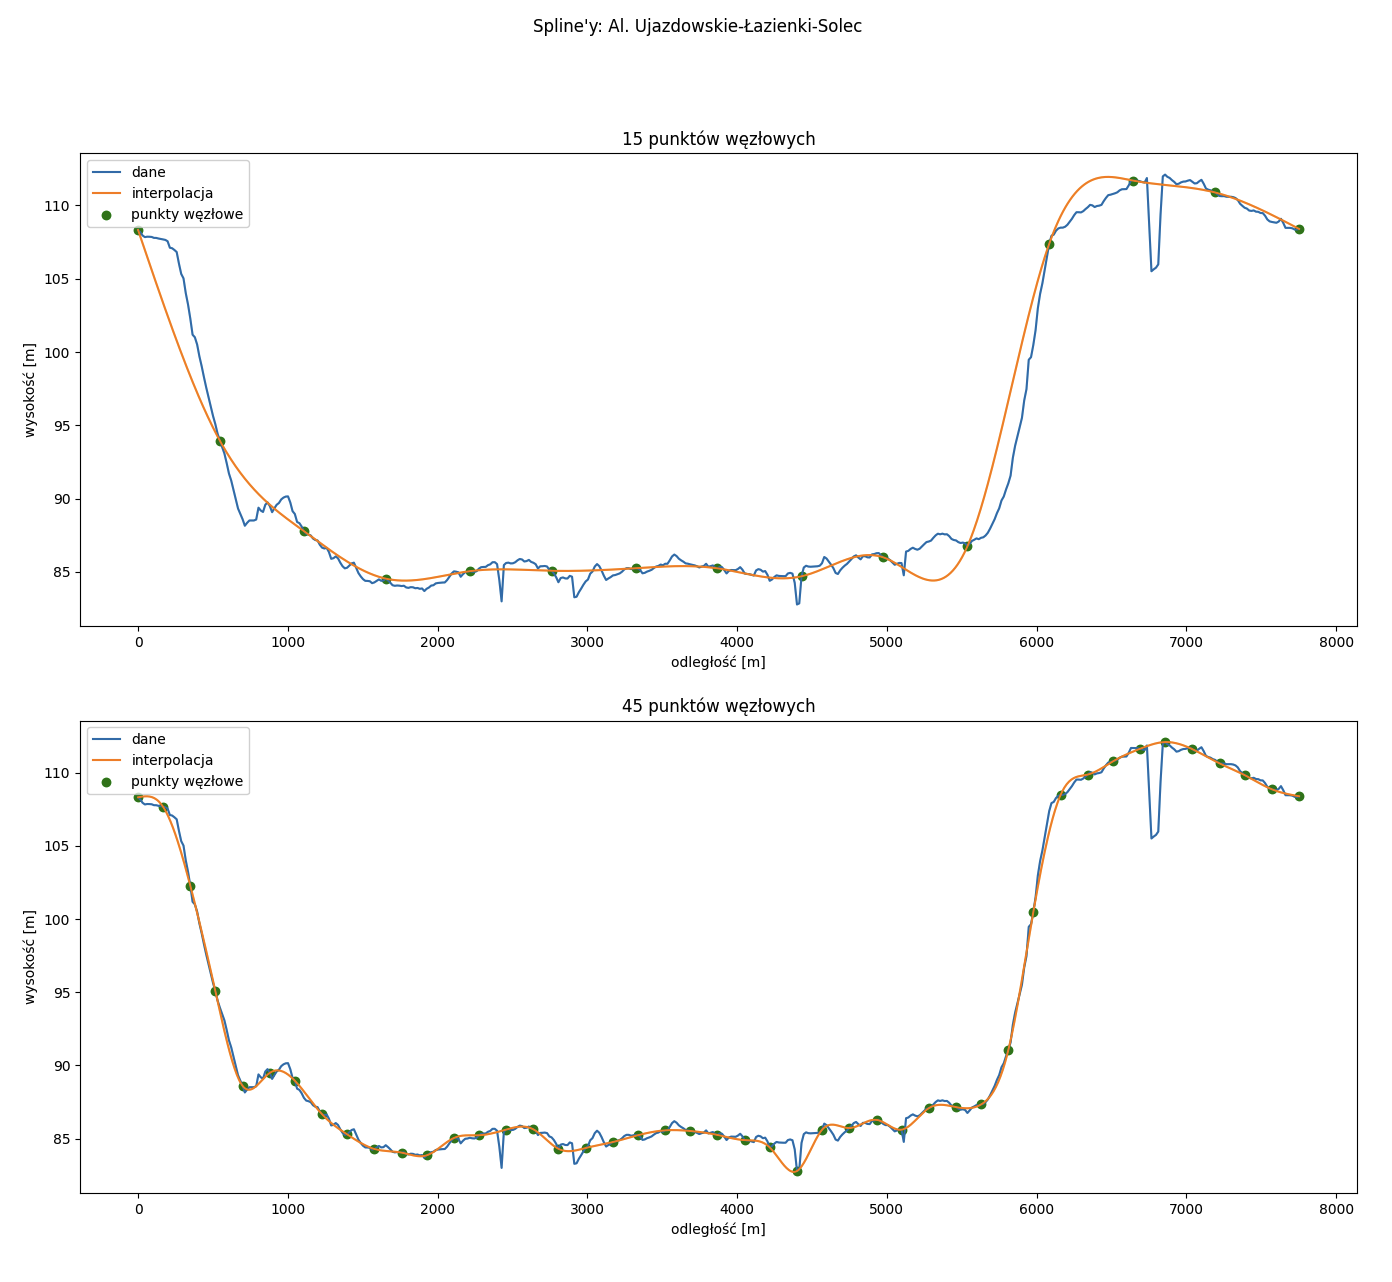
\includegraphics[width=12cm]{spline_wwa_uniform}
\end{center}
Dla metody krzywych sklejanych dla 15 punktów problem stanowią drobne oscylacje wysokości występujące po środku przedziału, dla tej metody możemy jednak
pozwolić sobie na \textbf{zwiększenie liczby punktów węzłowych} dzięki czemu otrzymujemy lepsze przybliżenie tych \textbf{chwilowych przeskoków} jak widać dla 45 węzłów. Warto zwrócić uwagę, że dla góry Fuji, w której profilu wysokościowym było mniej "szumu" bardzo dobrą interpolację osiągaliśmy dla mniejszej ilości punktów.
Zauważmy też, że \textbf{zaobserwowane dla mniejszej ilości punktów "wygładzenie" może być pożądanym efektem na przykład w przetwarzaniu sygnałów}.
Mimo wszystko, w przeciwieństwie do metody z wielomianem Lagrange'a, metodzie krzywych sklejanych udaje się osiągnąć dla tego terenu dobre rezultaty.
\section{Trasa wokół centrum Słupska}
 \begin{center}
	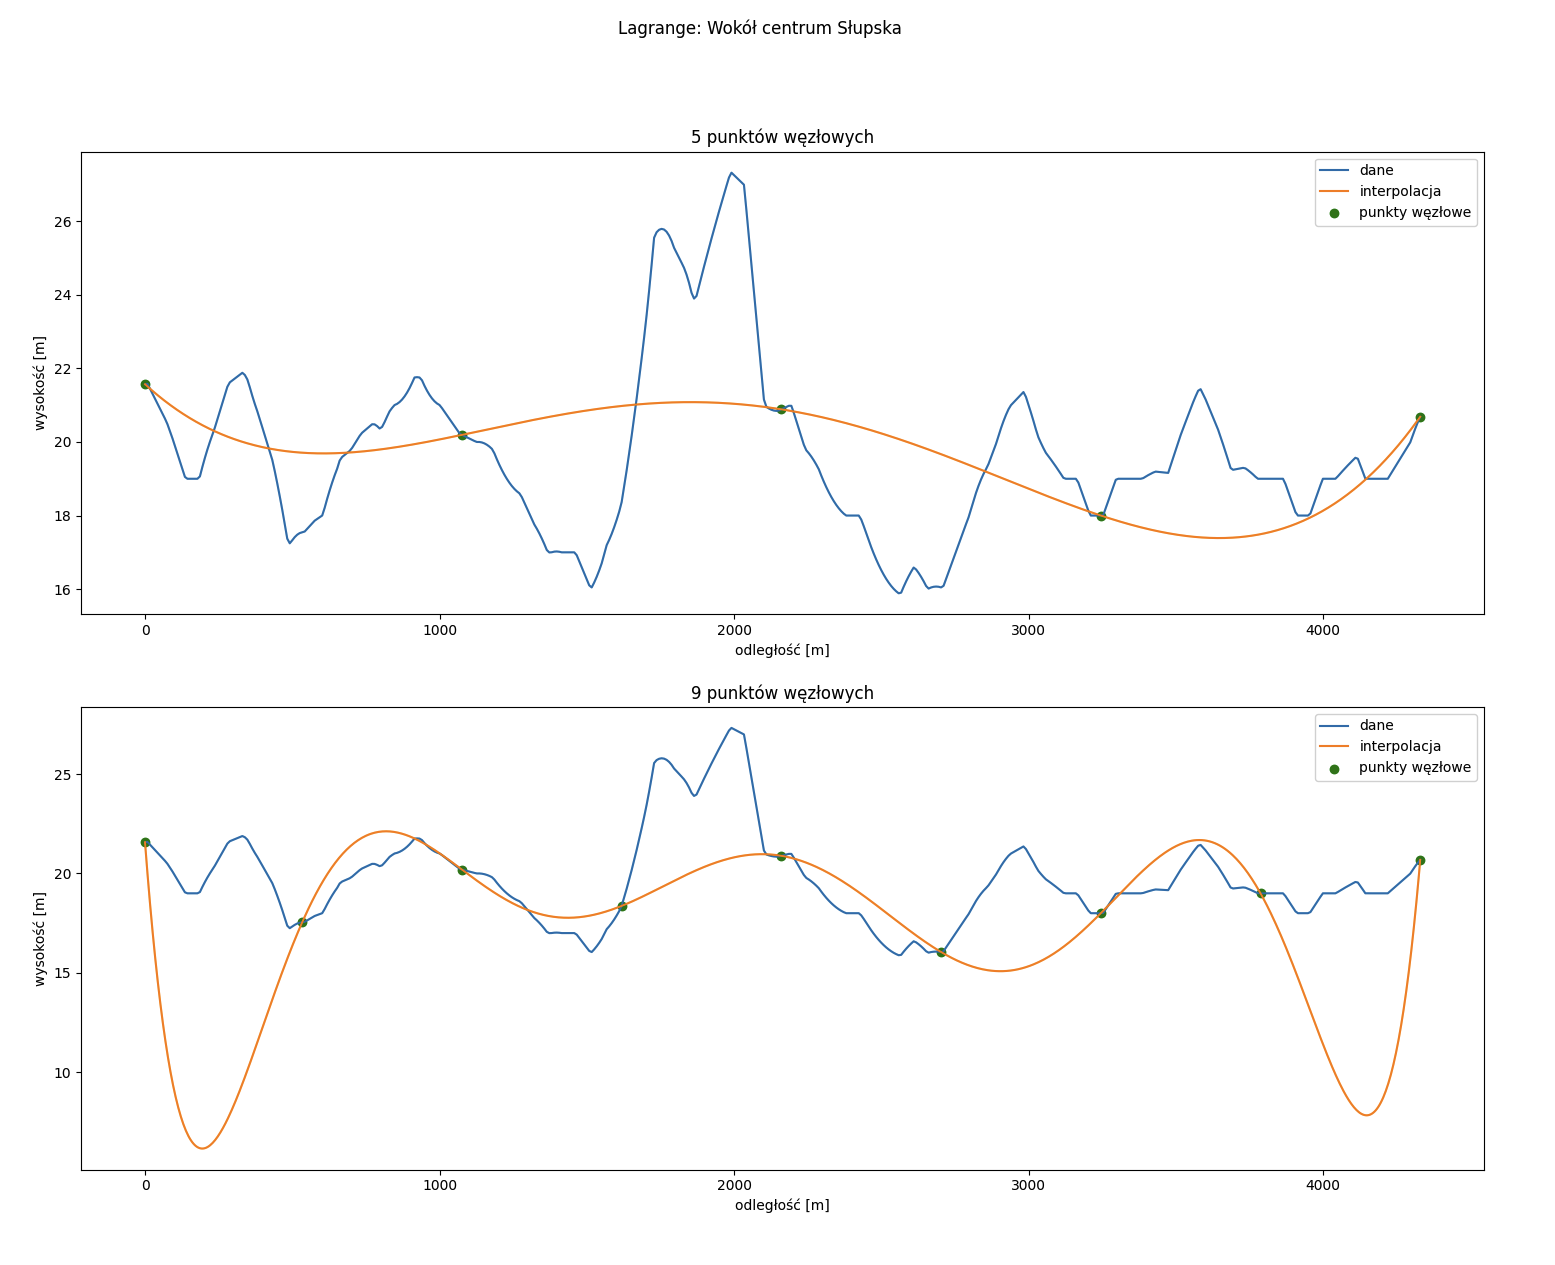
\includegraphics[width=12cm]{lagrange_slupsk_uniform}
\end{center}
Ostatni analizowany profil wysokościowy jest bardzo nieregularny, przy czym są to nagłe i gwałtowne spadki i wzrosty nachylenia.  Jak widać, w tym wypadku
duży efekt Rungego występuje już przy 9 węzłach, zatem jak wcześniej podejrzewaliśmy \textbf{na oscylacje wpływa nie tylko ilość punktów węzłowych ale także charakter
przebiegu interpolowanej funkcji}. Dla 5 węzłów mamy natomiast demonstrację, dlaczego dla nieregularnych funkcji potrzebujemy większej ilości punktów węzłowych w celu
otrzymania dobrej interpolacji - \textbf{zbyt mała ilość "próbek" nie zapewnia wystarczającej ilości informacji do odwzorowania profilu}. \\\\
Na poniższych wykresach natomiast widać zauważony już wcześniej wzrost oscylacji w środku przedziału przy zwiększaniu gęstości węzłów na krańcach przedziału.
Podobnego efektu nie ma dla metody krzywych sklejanych.
 \begin{center}
	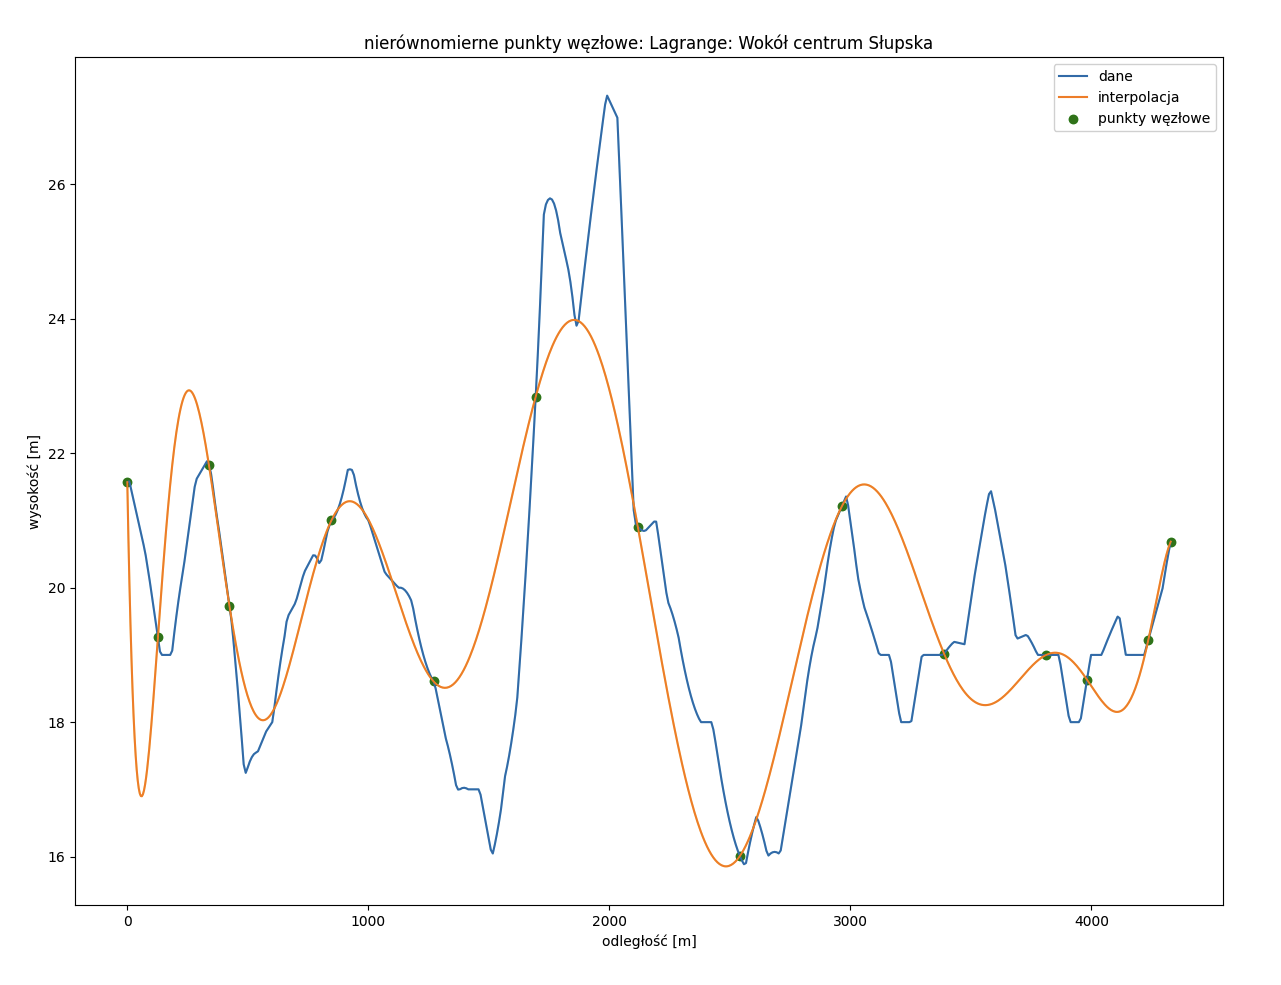
\includegraphics[width=8cm]{lagrange_slupsk_krance1}
\end{center}
 \begin{center}
	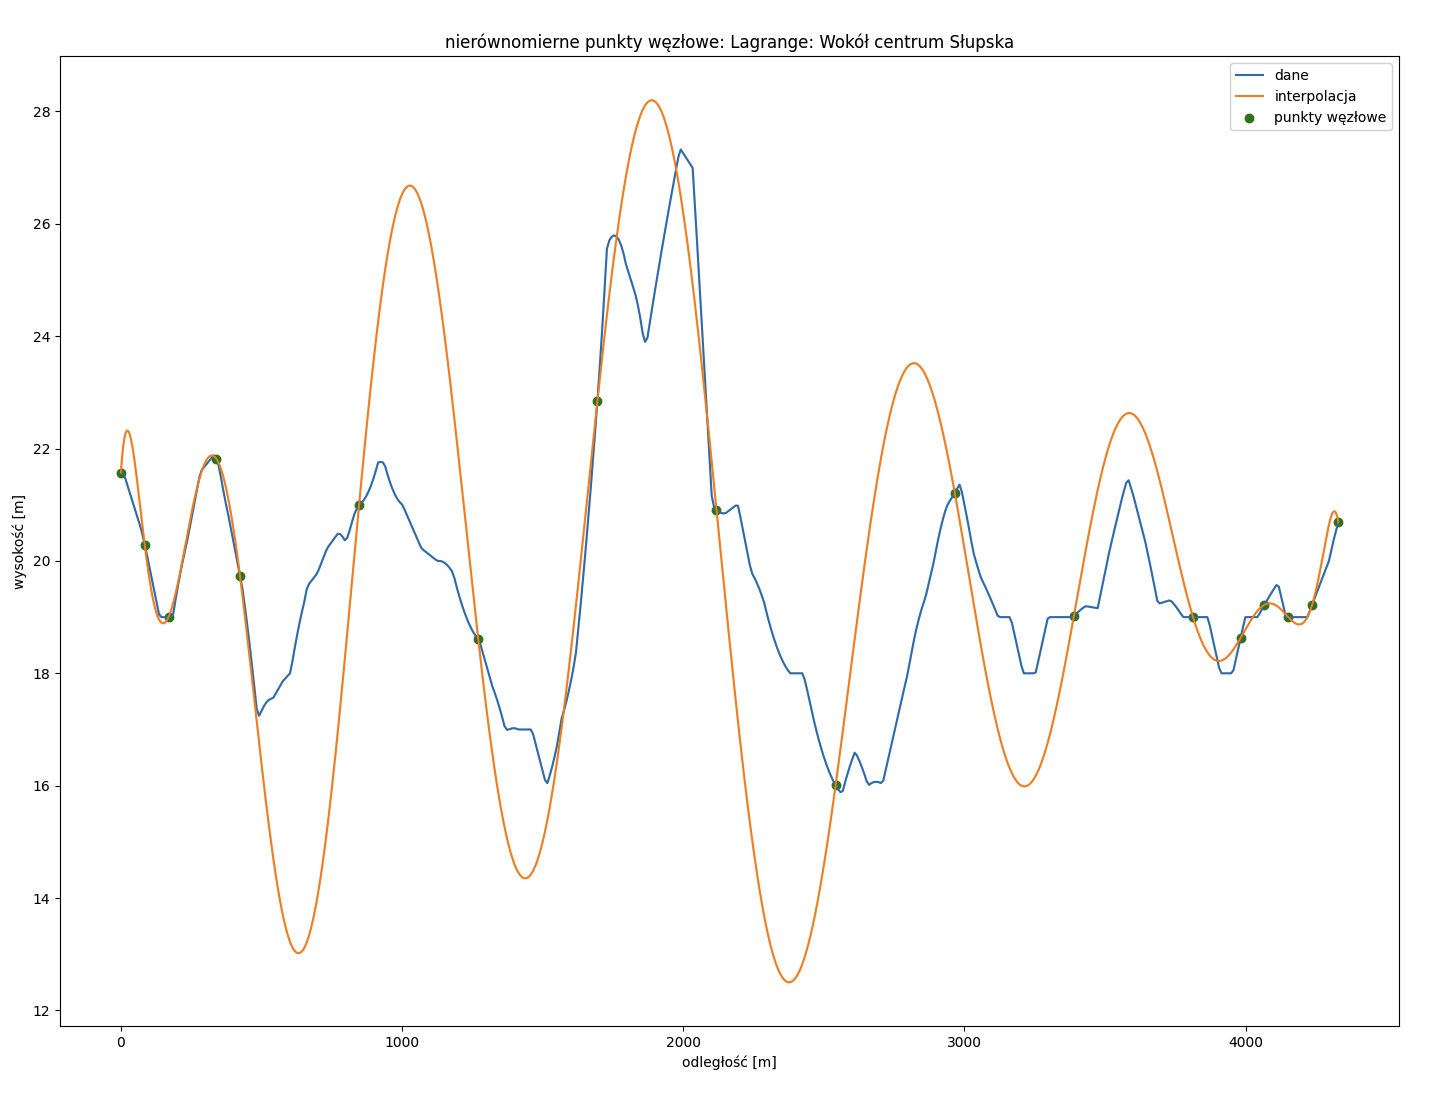
\includegraphics[width=8cm]{lagrange_slupsk_krance2}
\end{center}
 \begin{center}
	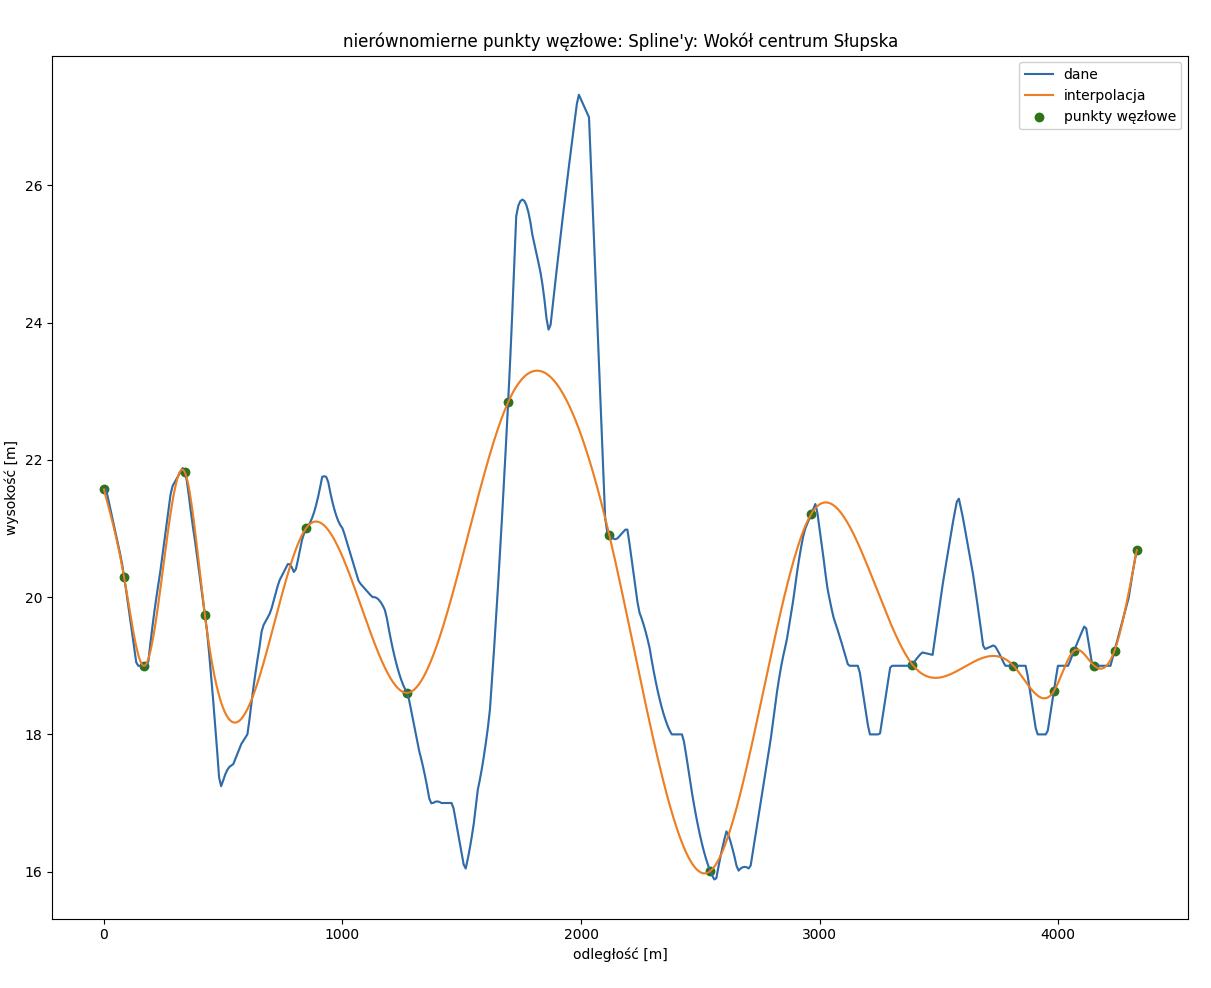
\includegraphics[width=8cm]{spline_slupsk_krance}
\end{center}
\section{Eliminacja efektu Rungego}
We wszystkich powyższych podpunktach głównym problemem metody interpolacji wielomianowej był efekt Rungego. Doszliśmy do wniosku, że istnieje 
pewna zależność między rozmieszczeniem punktów węzłowych a nasileniem tego efektu. Czy jesteśmy zatem w stanie określić tą zależność w celu wyznaczenia
rozmieszczenia węzłów, które pozwoli nam na niwelację efektu Rungego? Okazuje się, że tak! Dla $n$ punktów węzłowych ich rozmieszczenie będzie pokrywało się
z pierwiastkami wielomianu Czebyszewa stopnia $n$:
\begin{gather*}
	T_n(x) = cos(narccos x), x \in [-1, 1]
\end{gather*}
pierwiastki te są postaci
\begin{gather*}
	x_k = cos(\frac{2k+1}{2n} \pi), k= 0..n-1
\end{gather*}
rozmieścimy teraz węzły zgodnie z powyższym wzorem dla przypadku, w których efekt Rungego był najbardziej nasilony czyli trasy wokół centrum Słupska
 \begin{center}
	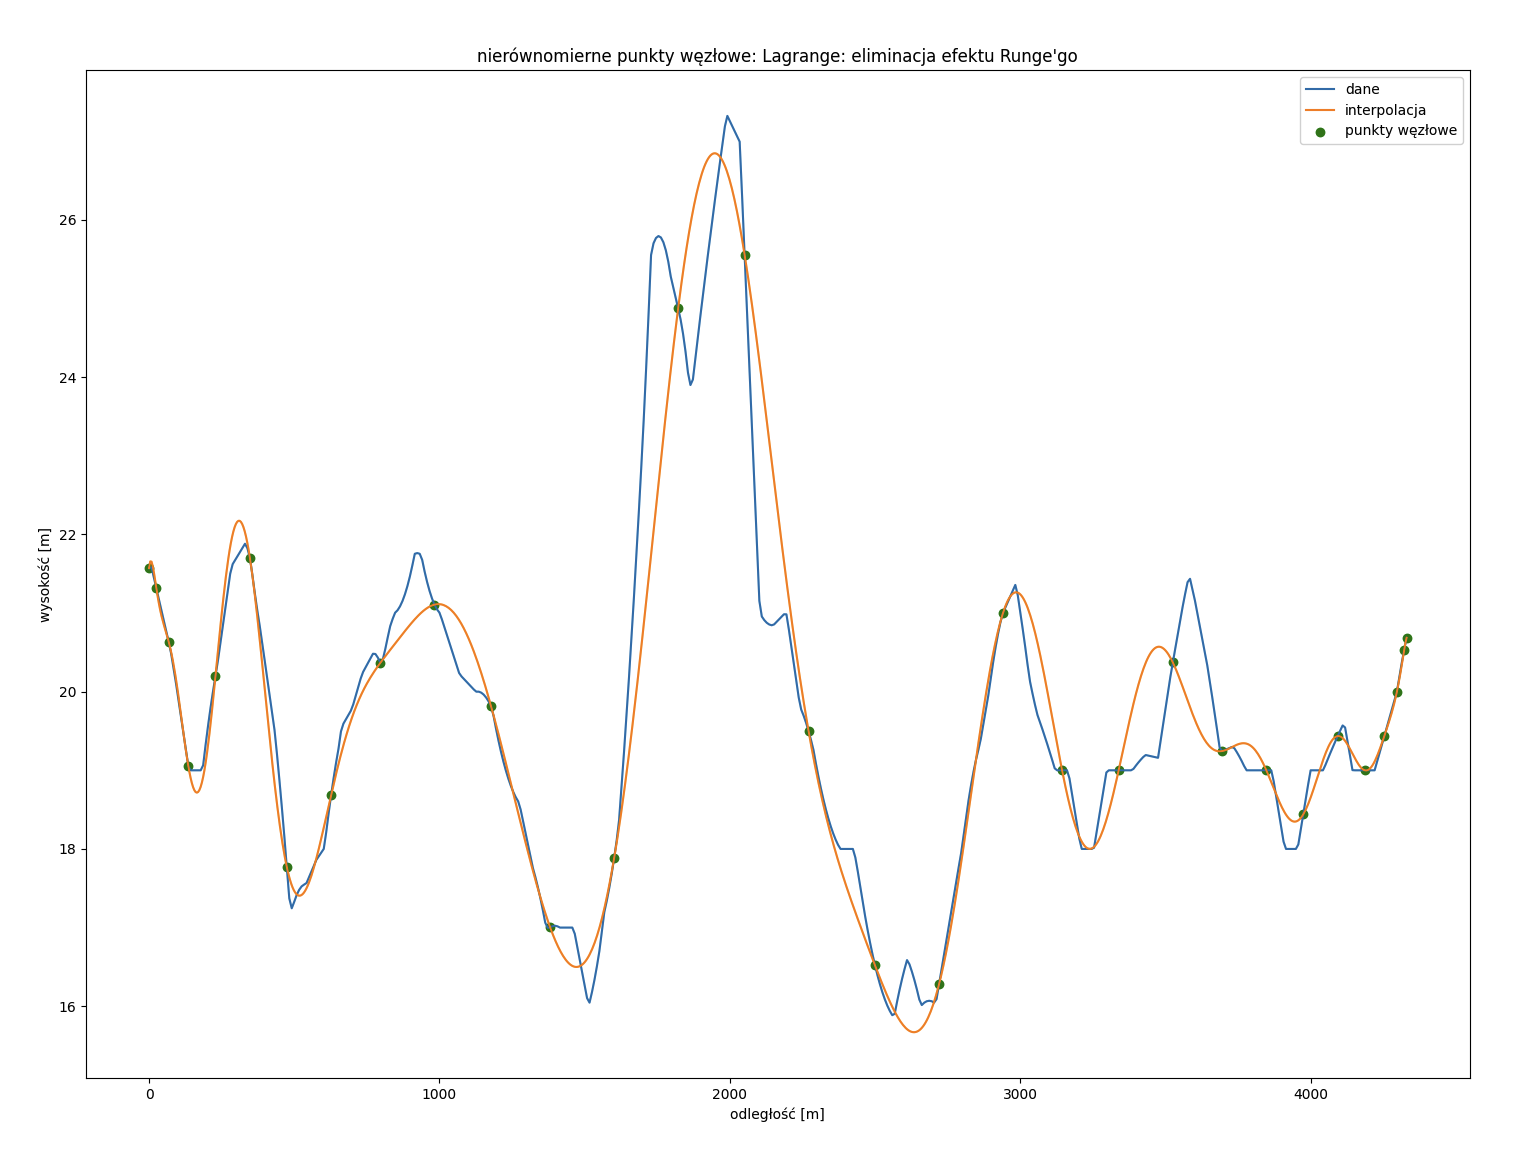
\includegraphics[width=8cm]{lagrange_runge_gone}
\end{center}
jak widać efekt Rungego został wyeliminowany, natomiast interpolacja jest gorsza niż gdyby użyć krzywych sklejanych dla 31 punktów:
 \begin{center}
	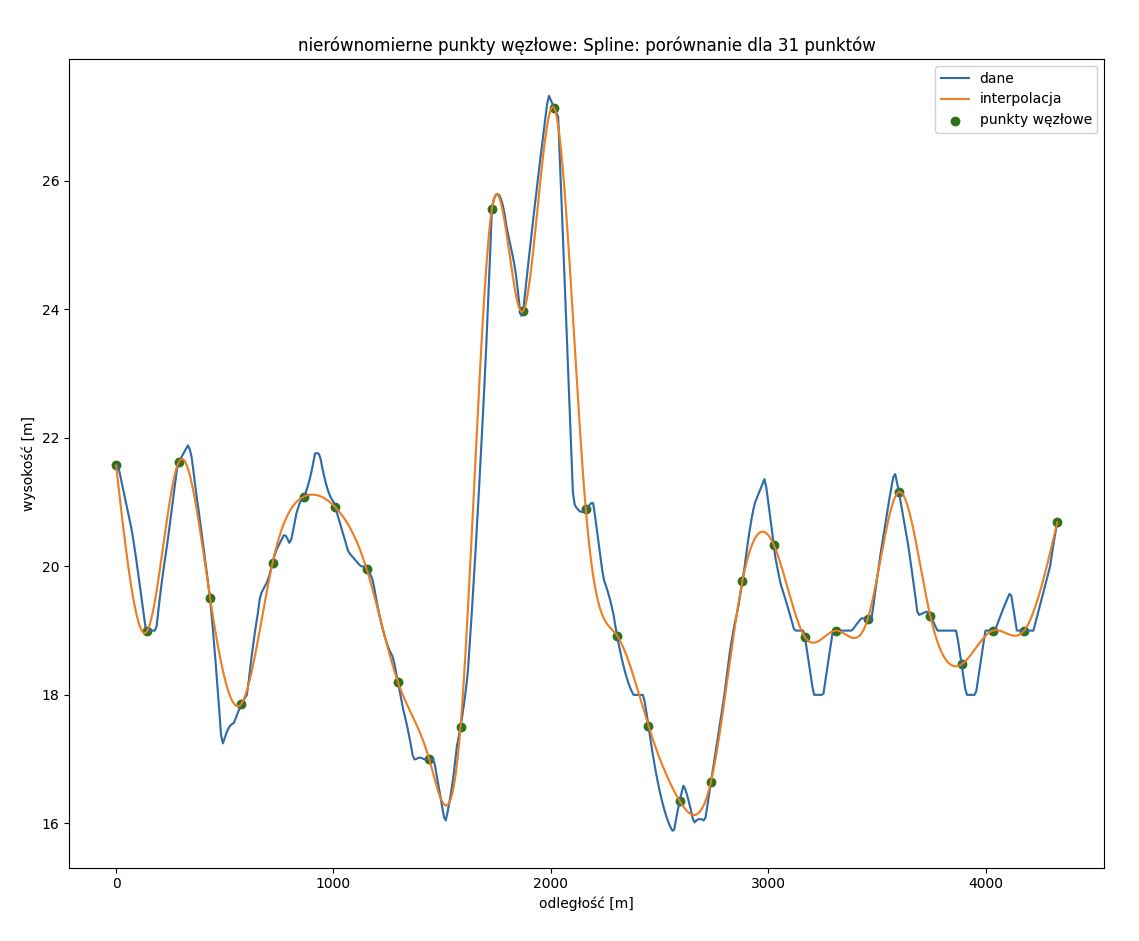
\includegraphics[width=8cm]{spline_runge_comparison}
\end{center}
dlatego nawet jeśli udało nam się pozbyć efektu Rungego należałoby się zastanowić czy nie lepiej dla naszego zastosowania użyć mimo wszystko krzywych sklejanych.
\section{Podsumowanie}
\section{Źródła}
\begin{itemize}
	\item \href{https://en.wikipedia.org/w/index.php?title=Spline_%28mathematics%29&oldid=288288033#Algorithm_for_computing_natural_cubic_splines}{Wikipedia-Spline}
	\item \href{https://medium.com/eatpredlove/natural-cubic-splines-implementation-with-python-edf68feb57aa}{Medium-Spline}
	\item \href{https://pl.wikipedia.org/wiki/Efekt_Rungego}{Efekt-Rungego}
	\item \href{https://byc-matematykiem.pl/tajniki-interpolacji-czesc-9/}{Węzły Czebyszewa}
\end{itemize}

\end{document}


